\section{Toy Models}

Let us examine some simple model systems proposed by Tully to help us understand the Trajectory Surface Hopping method.\cite{tully_1} 

\subsection{Simple Avoided Crossing}

The first system of our interest is a two level Hamiltonian characterized by a parameter $x$ in the diabatic representation is given below:

    \begin{equation} \label{simpleavoided}
        \mathcal{H}(x) = 
        \begin{pmatrix}
            \text{H}_{11}(x) & \text{H}_{12}(x) \\
            \text{H}_{21}(x) & \text{H}_{22}(x)
        \end{pmatrix}
    \end{equation}
where the matrix entries are:
    \begin{align*}
        \text{H}_{11}(x) &=  \begin{cases} \text{A}\left[1-\text{exp}(-\text{B}x)\right] & x > 0  \\ -\text{A}[1-\text{exp}(\text{B}x)] & x < 0 \end{cases} \\
        \text{H}_{12}(x) &= \text{H}_{21}(x) = \text{C}\text{exp}(-\text{D}x^2) \quad
        \text{H}_{22}(x) = -\text{H}_{11}(x)
    \end{align*}

The potential energy surfaces(PES) is obtained by diagonalising the Hamiltonian(adiabatic basis) in \eqref{simpleavoided} as a function of parameter $x$. PES is plotted in the figure below. The model is known as an avoided crossing because the energy surfaces at $x=0$ repel each other, i.e., they cannot cross each other. 
    
    \begin{figure}[H]
        \begin{center}
        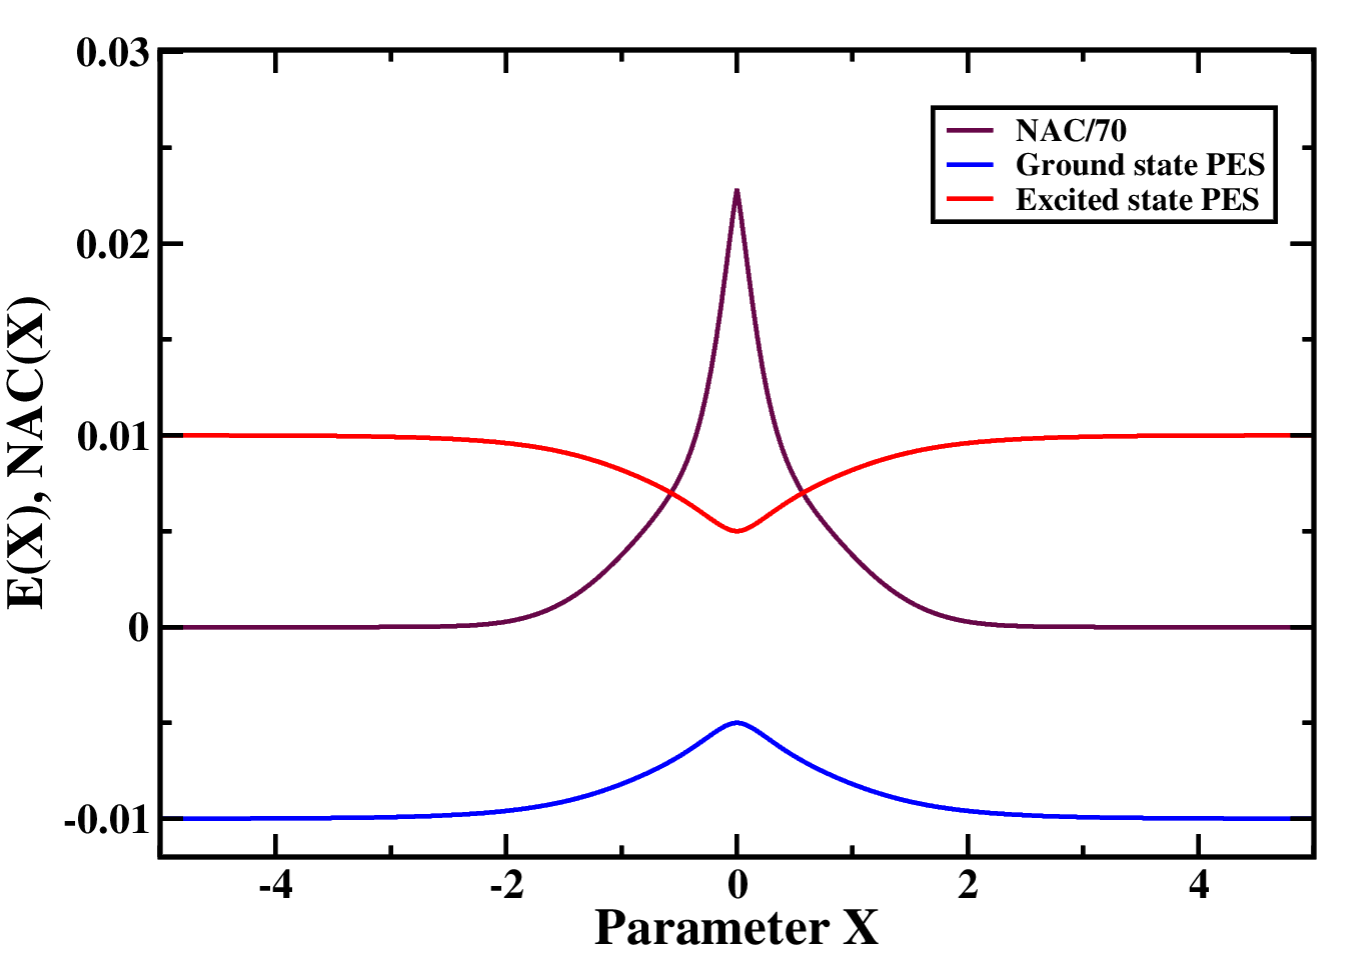
\includegraphics[width = 0.45\textwidth]{images/NAC.png}
        \end{center}
        \caption{Potential energy surfaces and the non-adiabatic coupling for simple avoided crossing}
        \label{fig:PES_Simpleavoided}
    \end{figure}

We also visualize one of the components of non-adiabatic coupling(NAC) vector plotted in \ref{fig:PES_Simpleavoided}. As discussed before, the NAC quantitatively gives us the strength of non-adiabatic transitions. Thus, we expect to see such transitions around $x=0$. Let us use Trajectory Surface Hopping to determine non-adiabatic transition probabilities of the trajectories initiated in asymptotic negative $x$ region of the ground state as a function of its momenta. The probabilities are obtained by keeping track of trajectories. The results are plotted below:
\begin{figure}[H]
\minipage{0.45\textwidth}
  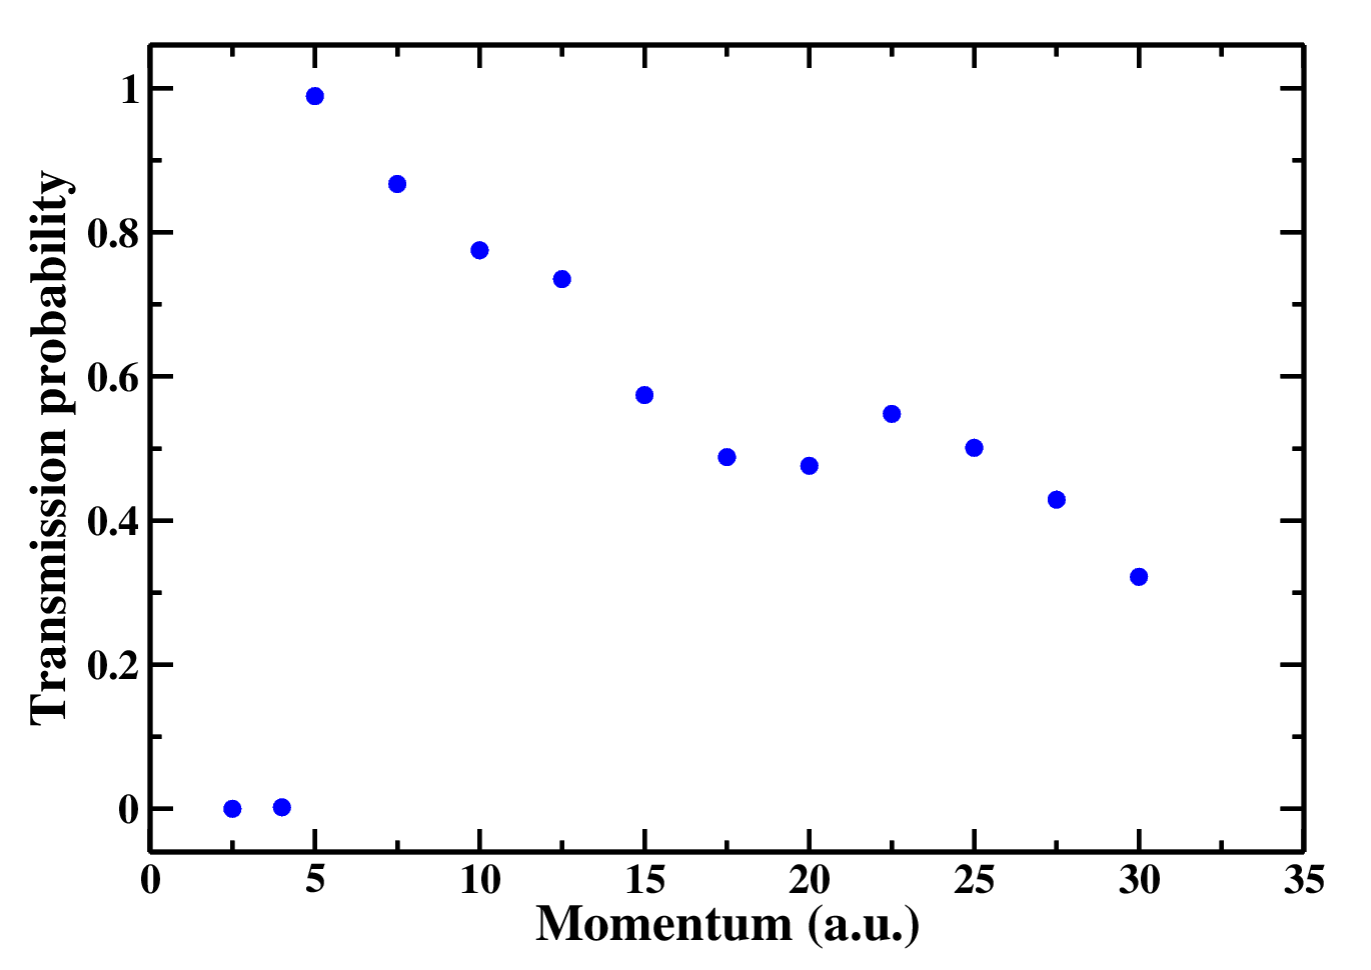
\includegraphics[width=1.1\linewidth]{images/Transmission_prob.png}
  \label{fig:transmission_prob}
  %\caption{A really Awesome Image}\label{fig:awesome_image1}
\endminipage \hspace{1.5em}
\minipage{0.45\textwidth}
  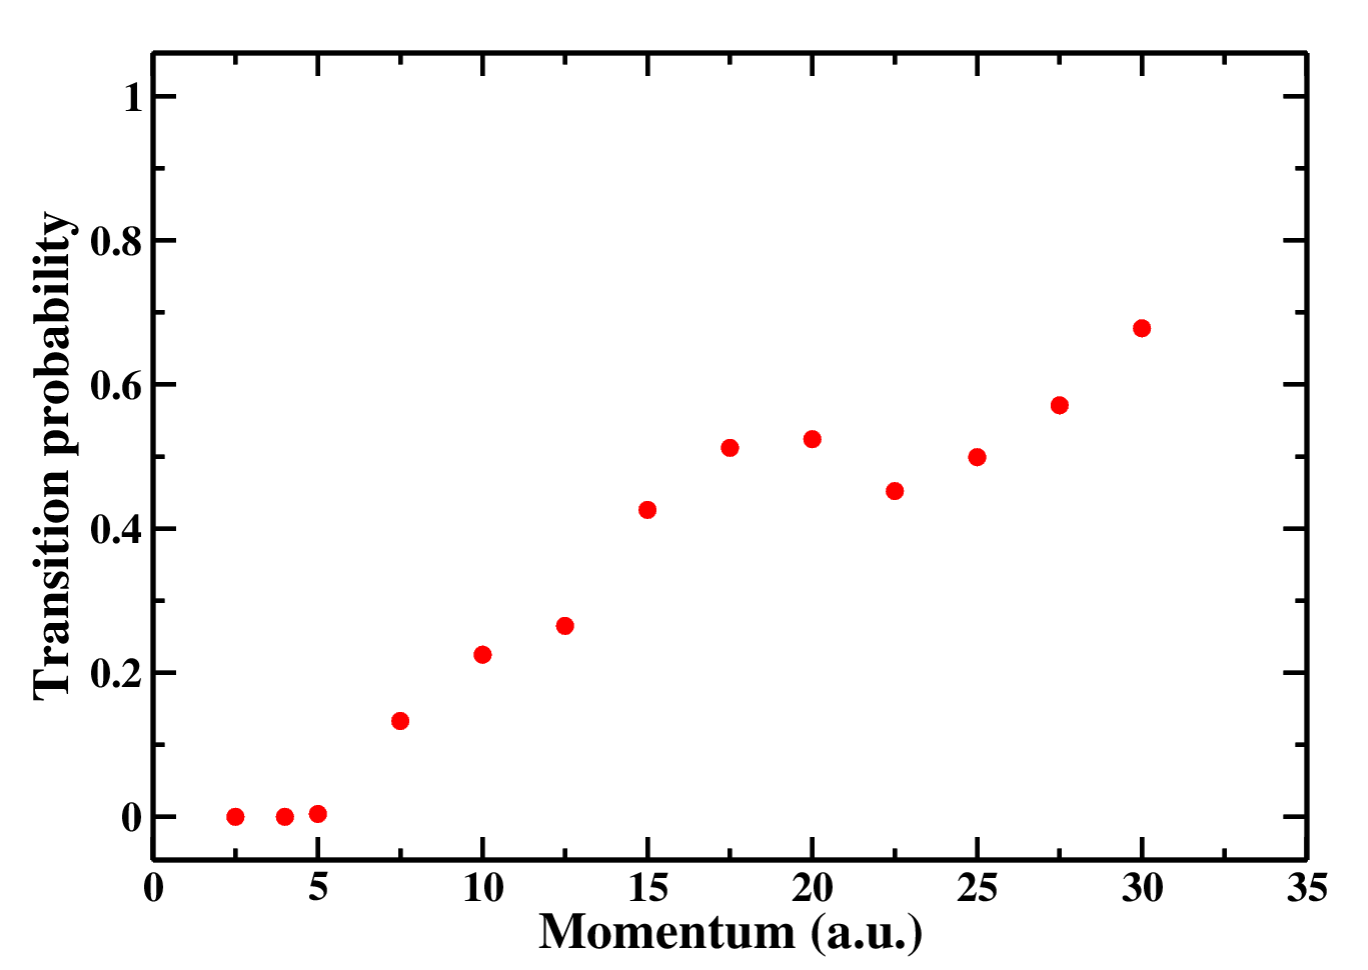
\includegraphics[width=1.1\linewidth]{images/Transition_prob.png}
  \label{fig:transition_prob}
  %\caption{A really Awesome Image}\label{fig:awesome_image2}
\endminipage\hfill
\caption{Transmission probability on the same surface(left) and transition probability(right) as a function of momentum of trajectories}
\label{Transmission and non-adiabatic transition probabilites}
\end{figure}
The most important observation is that we get transitions from the ground state to excited state which is shown in \ref{fig:transition_prob}. We can make an analogy to a diatomic molecule with the parameter $x$ being inter-nuclear distance. This analogy reveals that coupling between nuclear and electronic degrees of freedom can cause atomic transitions to different PES. \\ \\ For low momentum values, the nuclear trajectory cannot overcome the barrier around $x=0$ due to its classical nature in TSH. As its momentum is increased, the probability of transmission across the barrier increases as the energy increases. A further increase in momentum, we see a rise in transition probability and reduce in transmission as expected intuitively. These results are in very good agreement with quantum calculations except a small deviations for low momentum values due to tunnelling.
%\subsection{Extended coupling with Reflection}

\section{Conclusion}

As described above, the trajectory surface hopping simulations capture the non-adiabatic transitions and even agree with quantum calculations well within the statistical error. Also, the conceptual simplicity aids in its popular tool to study non-adiabatic dynamics. However there are certain fundamental problems with TSH. First, the inherent assumption of treating nucleus classically lead to inconsistencies. It cannot describe processes such as nuclear tunneling and dephasing.\cite{curchod,dephasing_1,dephasing_2} Second, surface hopping scheme leads to over-coherences of electronic coefficients over long time which may qualititavely degrade the results.\cite{coherences,wang_TSH} Also, energy should be conserved during the simulation and the velocity is re-adjusted to fulfill this criterion. If the energy conservation cannot be met, a frustrated hop occurs and the standard way is to keep the trajectory unchanged. However, this procedure can lead to a completely different behaviour if a frustrated hop occurs at the crossings. A lot of proposals and work has been done to overcome the shortcomings.\cite{TSH_review,dephasing_2,gen_tsh,quantum_tsh} \\ \\ 
We have successfully written a python wrapper over NWChem platform to simulate non-adiabatic dynamics through TSH. We need to test and benchmark it on different molecular systems. There is a scope for lot of improvement in the code. Our future plans include parallelization of the code to distribute it over nodes. Also, the performance can be improved by replacing the code for crucial parts by a compiled programming language than Python. Apart from performance related issues, the code can be furthered developed to incorporate more functionality to overcome the above problems and also more physics including Spin-Orbit coupling, Floquet formalism for periodic potential, etc.\cite{TSH_review}